\documentclass[11pt,a4paper]{article}
\usepackage[margin=0.75in]{geometry}
\usepackage{graphicx}
\usepackage{authblk}
\usepackage{subcaption}
\usepackage{tikz}
\usepackage{amsmath}
\usepackage{amssymb}
\usepackage{hyperref}

\usetikzlibrary{positioning,arrows.meta}

\author[1]{Santiago Acosta\thanks{santiago\_acosta@ucsb.edu}}
\author[1]{Jonathan Skaza\thanks{skaza@ucsb.edu\\Code available at: \texttt{https://github.com/jskaza/Neural-Population-Geometry}}}
\affil[1]{Dynamical Neuroscience Graduate Program, University of California, Santa Barbara}
\title {Neural Population Geometry \\[1ex] \large ME 225NN, Winter 2025}
\date{}

\begin{document}
\maketitle
\section{Introduction}

\subsection{Problem Description \& Motivation}
Experimental neuroscience has seen rapid advances in recording techniques, enabling simultaneous recordings from thousands of neurons (and potentially up to a million~\cite{demas2021high}). These technological breakthroughs have driven theoretical neuroscientists to develop new methodologies for analyzing neural populations. Such large-scale analyses face distinct challenges: neurons typically respond to multiple variables simultaneously, complicating functional interpretation, while real-world tasks require robustness to complex variability that traditional tuning-based approaches struggle to capture.

In consideration of these factors, the focus of neural population analysis has transitioned from single-neuron tuning to \textit{geometric} approaches that consider population-level representations~\cite{yuste2015neuron, saxena2019towards}. Traditional single-neuron tuning approaches characterize individual neurons by their response profiles to specific stimuli or task variables. For example, in the visual cortex, neurons might be classified by their preferred orientation, spatial frequency, or direction of motion, while in the motor cortex, neurons might be described by their correlation with movement direction or force. This approach, pioneered by Hubel and Wiesel's work on the visual cortex~\cite{hubel1959receptive}, has been instrumental in mapping functional properties across brain regions but struggles to capture the complex, multi-dimensional nature of neural responses during naturalistic behaviors.

The rationale behind the shift to population-level analysis is that neural computations emerge from structured, high-dimensional activity patterns rather than isolated responses of individual neurons. These patterns are conceptualized as \textit{neural manifolds}---low-dimensional geometric structures embedded in high-dimensional neural state space. The geometric properties of these manifolds---dimensionality, curvature, separability, and capacity (the number of distinct manifolds a neural system can support)---reveal computational principles governing neuronal networks~\cite{chung2021neural}. 

A compelling aspect of the neural manifold framework is its ability to link geometric structures to specific behavioral or cognitive variables. For example, ring-shaped manifolds have been observed in the mammalian hippocampus encoding head direction~\cite{chaudhuri2019intrinsic} and in the mouse visual cortex representing stimulus orientation~\cite{beshkov2024topological}. These direct mappings between manifold geometry and task variables provide mechanistic insights into how neural populations encode and process information relevant to behavior.

This report examines the application of geometric techniques to analyze large neuronal populations—a field known as \textit{neural population geometry}. This framework provides a unified approach for understanding both biological neural circuits and artificial neural networks (ANNs). By conceptualizing neural computation as geometric transformations, we can analyze how population-level representations enable robust, efficient, and scalable information processing across biological and artificial systems. This parallel analysis reveals fundamental computational principles that transcend the specific implementation details of different neural architectures.

\subsection{Literature Review}
\subsection{Summary}
In this paper, we demonstrate how neural population geometry provides a unified framework for understanding information encoding in both biological and artificial neural systems. We focus specifically on the representation of circular variables—a fundamental computational challenge that requires preserving topological structure. Through parallel analyses of orientation encoding in the mouse visual cortex and a trained convolutional neural network (CNN), we show how similar ring-shaped manifolds emerge in both systems despite their different implementations.

Our analysis reveals that these circular manifolds arise naturally from the computational demands of the task rather than from specific architectural constraints. In the mouse visual cortex, we characterize how populations of neurons collectively form a ring-shaped manifold that encodes orientation information, with the manifold's geometry reflecting the circular topology of orientation space. Similarly, in our CNN simulation, we demonstrate how the network spontaneously develops a circular representation in its latent space when trained to discriminate orientation angles.

By comparing the geometric properties of these representations---including dimensionality, curvature, and topological structure---we identify common principles that govern how neural systems, both biological and artificial, efficiently encode circular variables. This comparative approach highlights how neural population geometry can be applied to both neuroscience and machine learning, offering insights into fundamental computational strategies that transcend specific neural implementations.

\section{Preliminaries}

\subsection{Mathematical Foundations of Neural Manifolds}

In mathematics, a \textit{manifold} is a topological space that locally resembles Euclidean space. Formally, an $m$-dimensional manifold $\mathcal{M}$ is a topological space where each point $p \in \mathcal{M}$ has a neighborhood $U$ that is homeomorphic to an open subset of $\mathbb{R}^m$. 

In neuroscience, the concept of a \textit{neural manifold} extends this mathematical definition to describe geometric structures in neural population activity ( Fig.~\ref{fig:manifolds}). Consider a population of $n$ neurons, where the activity of each neuron can be represented as a coordinate in an $n$-dimensional neural state space $\mathbb{R}^n$. Let $\mathbf{r} = (r_1, r_2, \ldots, r_n) \in \mathbb{R}^n$ represent the firing rates of these neurons at a given time. The neural manifold hypothesis posits that, during specific task execution, these population activity patterns do not explore the entire $n$-dimensional space but instead are constrained to a lower-dimensional subspace or manifold $\mathcal{M} \subset \mathbb{R}^n$, where typically $\dim(\mathcal{M}) \ll n$.

Formally, we can define a neural manifold as follows: Let $\mathbf{r}(t) \in \mathbb{R}^n$ represent the population activity at time $t$. For a given task or stimulus condition $s$ from a set of possible conditions $\mathcal{S}$, the neural manifold $\mathcal{M}_s$ is defined as:

\begin{equation}
\mathcal{M}_s = \{\mathbf{r}(t) \in \mathbb{R}^n : \text{condition } s \text{ is presented at time } t\}
\end{equation}

It is important to note that real neural data exhibits characteristics that extend beyond the strict mathematical definition of a manifold in two key ways:

\begin{enumerate}
    \item \textit{Neural variability}: When the same stimulus is presented repeatedly, neural responses vary due to stochastic processes in neural firing. This variability is thought to be fundamental to neural coding and transforms what would be a sparse set of isolated points (one per stimulus) into richer \textit{point clouds} (clusters of points for each stimulus). These point clouds collectively define the empirical neural manifold, with the distribution and statistical properties of responses containing important information about the neural code.
    
    \item \textit{Sparse sampling}: Experimental limitations often allow only a finite sampling of possible stimuli or conditions, providing discrete observations of what is theoretically a continuous underlying manifold structure.
\end{enumerate}

\subsection{Types of Neural Manifolds}

Several types of neural manifolds have been identified in neuroscience research:

\begin{enumerate}
    \item \textit{Object manifolds} or \textit{perceptual manifolds} arise in sensory neural populations as a result of identity-preserving variations in stimulus properties. For example, if $\mathbf{x} \in \mathbb{R}^d$ represents a stimulus (e.g., an image) and $T_\theta: \mathbb{R}^d \rightarrow \mathbb{R}^d$ represents a transformation with parameter $\theta$ (e.g., rotation), then the object manifold is defined as:
    
    \begin{equation}
    \mathcal{M}_{\text{obj}} = \{f(T_\theta(\mathbf{x})) : \theta \in \Theta\}
    \end{equation}
    
    where $f: \mathbb{R}^d \rightarrow \mathbb{R}^n$ represents the neural encoding function mapping stimuli to population responses, and $\Theta$ is the set of possible transformation parameters.
    
    \item \textit{Point-cloud manifolds} represent the empirical manifestation of neural manifolds in experimental data. Given a set of stimuli $\{s_1, s_2, \ldots, s_k\}$ and corresponding neural responses $\{\mathbf{r}_1, \mathbf{r}_2, \ldots, \mathbf{r}_k\}$, the point-cloud manifold is:
    
    \begin{equation}
    \hat{\mathcal{M}} = \{\mathbf{r}_i : i = 1, 2, \ldots, k\}
    \end{equation}
    
    This discrete set of points approximates the underlying continuous manifold structure, with the approximation quality depending on sampling density and noise levels.
    
    To estimate the continuous manifold from these discrete point clouds, several approaches have been developed that focus on uncovering the intrinsic geometry of neural representations~\cite{chung2021neural}:
    
    \begin{itemize}
        \item \textit{Linear dimensionality reduction}: Methods such as Principal Component Analysis (PCA) identify the shape, location, and orientation of neural data within the neural state space by providing a Cartesian coordinate basis describing subspaces in which the data lie. While computationally efficient, these methods can only capture linear subspaces and may miss important nonlinear structure in the data.
        
        \item \textit{Nonlinear dimensionality reduction}: To characterize the intrinsic geometry of neural manifolds, which are often curved and nonlinear, methods such as Isomap~\cite{tenenbaum2000global}, Locally Linear Embedding (LLE)~\cite{roweis2000nonlinear}, t-SNE~\cite{vandermaaten2008visualizing}, Multidimensional Scaling (MDS)~\cite{kruskal1964multidimensional}, PHATE~\cite{moon2019visualizing}, and UMAP~\cite{mcinnes2018umap} can be employed. These techniques attempt to preserve local or global geometric relationships in the data while reducing dimensionality. However, they typically assume topologically simple manifolds and may fail to capture complex topological structures.
        
        \item \textit{Topologically-motivated methods}: For neural data with complex topological structure, specialized techniques have been developed. Spline Parameterization for Unsupervised Decoding (SPUD)~\cite{chaudhuri2019intrinsic} uses cubic splines to parameterize low-dimensional manifolds, enabling the discovery of ring-shaped manifolds in head direction cells. This approach leverages persistent homology to determine the intrinsic dimension and uncover nontrivial topological structures in neural data.
        
        \item \textit{Dynamics-based approaches}: Methods like Manifold Inference from Neural Dynamics (MIND)~\cite{low2018probing} define distances between neural states based on transition probabilities, which gives rise to intrinsic dimensions relevant for topological maps underlying task implementation. This approach has been successfully applied to characterize neural activity in the hippocampus during spatial navigation tasks, revealing toroidal manifold structures in grid cells.
        
        \item \textit{Geometric approximation methods}: Traditional approaches such as convex hulls provide geometric approximations of the manifold boundary. While convex hulls offer a simple outer boundary by finding the smallest convex shape that completely encloses a set of points in a given space, they may miss ``holes''.
        
        \item \textit{Density-based approaches}: For noisy neural data, methods like kernel density estimation (KDE) create continuous representations by estimating the probability density function of the point cloud. The manifold boundary can then be defined as a level set of this density estimate, providing robustness to outliers and noise.
    \end{itemize}
    
    The choice of estimation method depends on the hypothesized structure of the neural manifold and the characteristics of the data. Linear methods are appropriate when the manifold is expected to be flat, while nonlinear methods are necessary for curved manifolds. Topologically-motivated methods are essential when the manifold has complex topology, such as circular or toroidal structures often found in neural representations of periodic variables like orientation or spatial location.
\end{enumerate}

\subsection{Neural Population Geometry}

Neural population geometry refers to the study of configurations, relationships, and properties of neural manifolds embedded in the high-dimensional neural state space. This framework provides quantitative measures to characterize neural representations:

\begin{enumerate}
    \item \textit{Dimensionality}: The intrinsic dimensionality $d$ of a neural manifold $\mathcal{M}$ can be estimated using techniques such as principal component analysis (PCA) or more sophisticated nonlinear dimensionality reduction methods.
    
    \item \textit{Curvature}: For a smooth manifold, the curvature at point $p \in \mathcal{M}$ quantifies how the manifold deviates from a flat Euclidean space locally. Intuitively, curvature measures how much a surface ``bends'' at a given point. In neural manifolds, regions of high curvature often represent areas where small changes in stimuli produce large changes in neural responses. This can be characterized mathematically using concepts like the second fundamental form or Ricci curvature, which provide formal ways to measure this bending in different directions.
    
    \item \textit{Separability}: For multiple manifolds $\mathcal{M}_1, \mathcal{M}_2, \ldots, \mathcal{M}_k$ corresponding to different stimulus conditions, separability measures how distinguishable these manifolds are. One metric is the minimum distance between manifolds:
    
    \begin{equation}
    d(\mathcal{M}_i, \mathcal{M}_j) = \min_{\mathbf{r}_i \in \mathcal{M}_i, \mathbf{r}_j \in \mathcal{M}_j} \|\mathbf{r}_i - \mathbf{r}_j\|
    \end{equation}
    
    \item \textit{Capacity}: The number of distinct manifolds a neural system can support, which relates to the information-carrying capacity of the population.
\end{enumerate}

The geometric properties of neural manifolds provide insights into the computational principles governing neural information processing, including how information is encoded, transformed, and decoded across neural circuits.

\begin{figure}
    \centering
    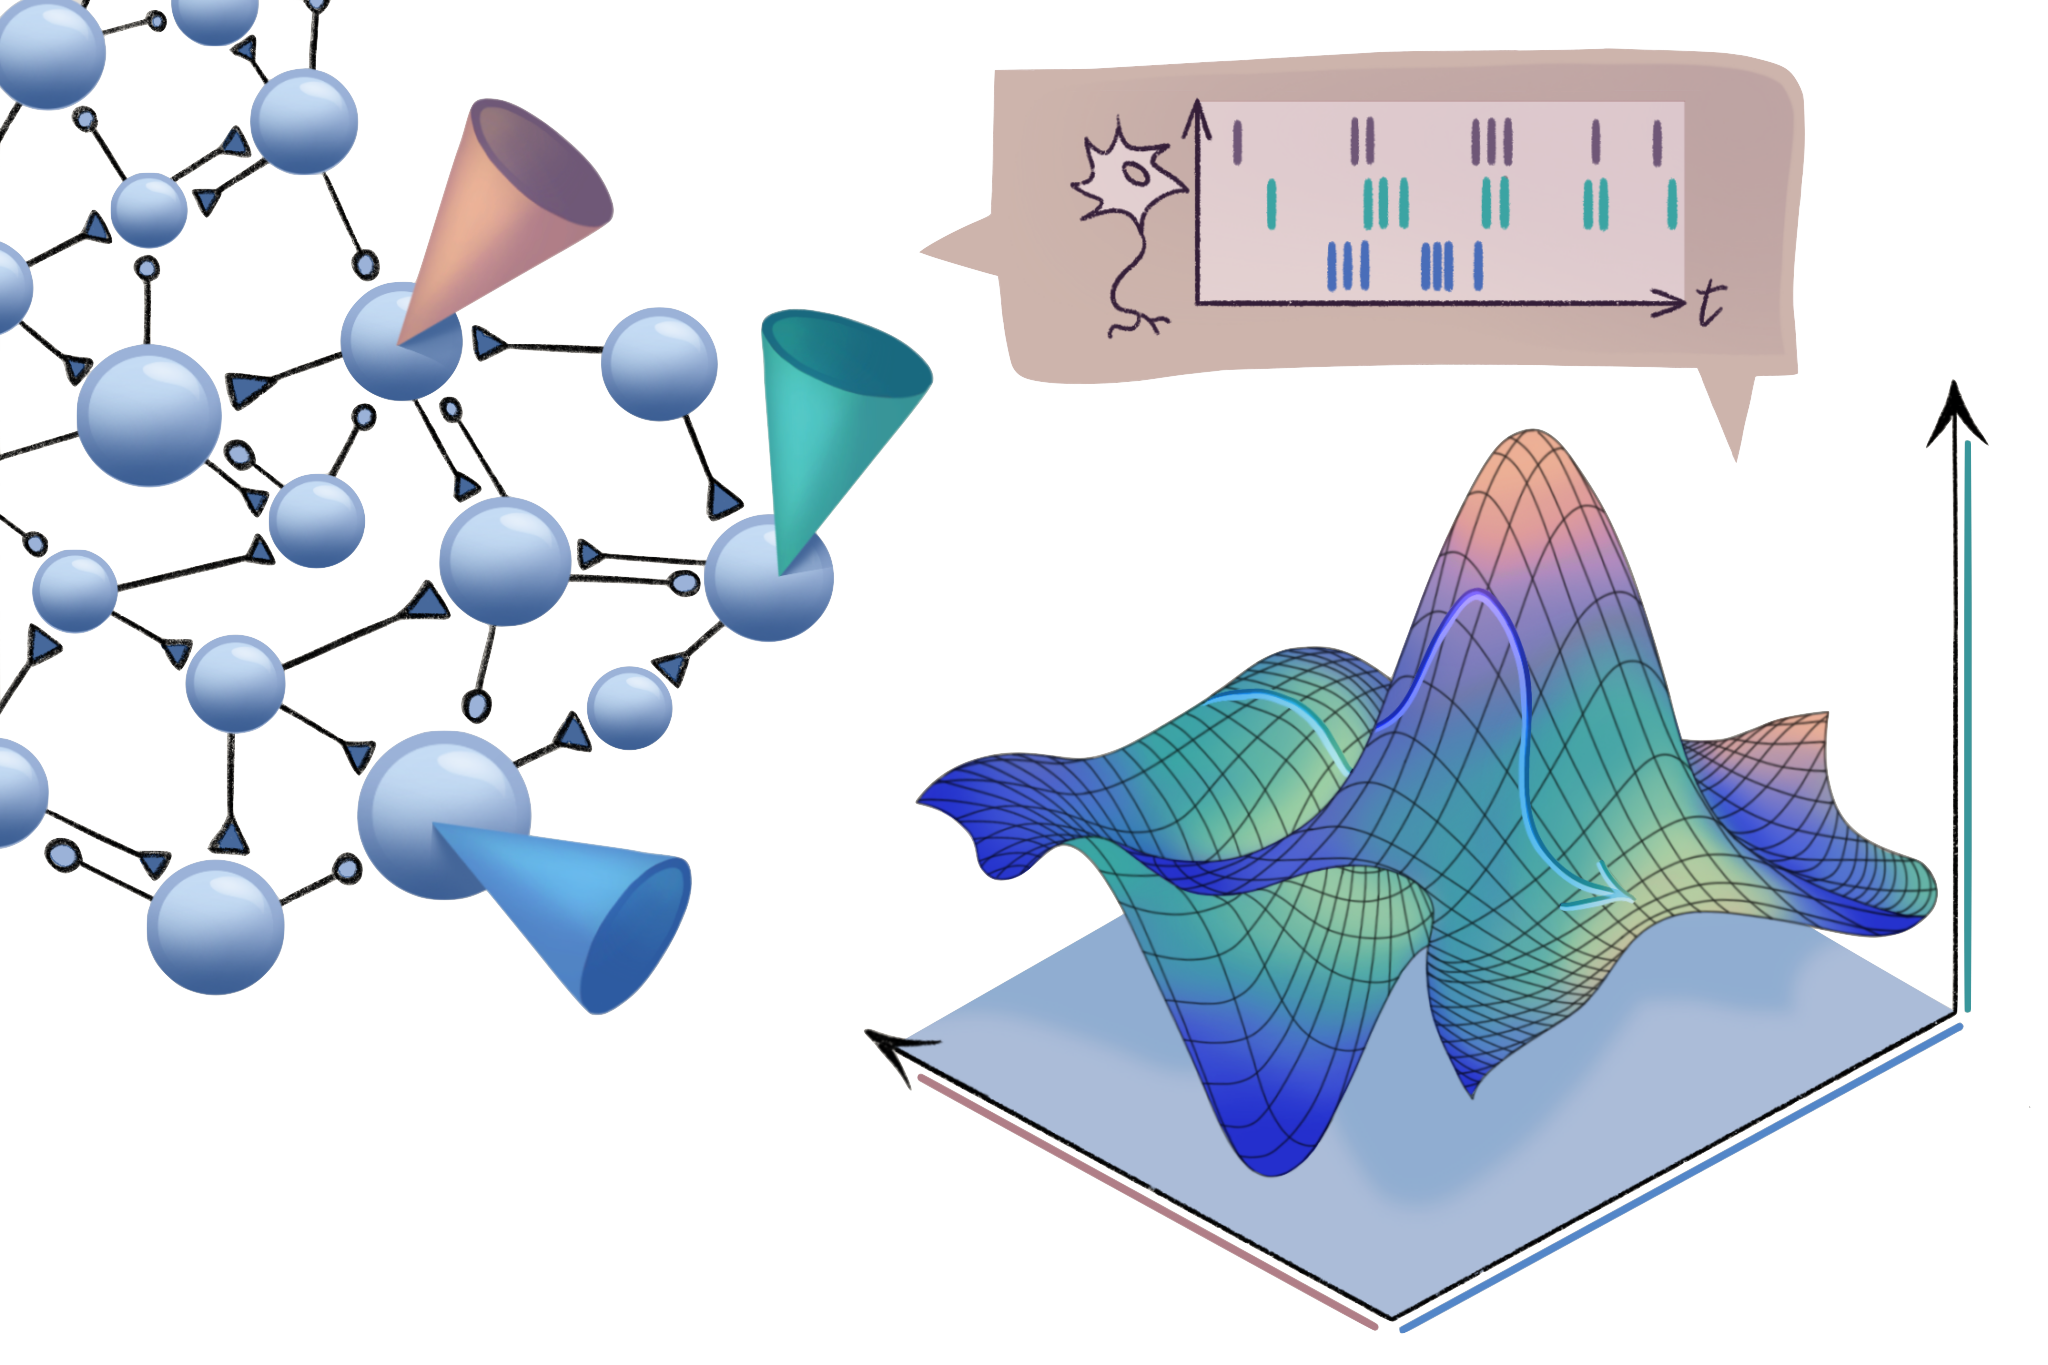
\includegraphics[width=0.75\linewidth]{figs/manifold_schematic.png}
    \caption{A neural manifold is formed by plotting neural activity (e.g., firing rate) in state space, where each axis is a single neuron. Note that the repeated presentation of the same stimulus does not lead to the occupancy of an identical point within the state space. Rather, neuronal variability induces fluctuations in the points derived from different trials. Consequently, each stimulus is associated not with a single point but with a point cloud, the dimensions and configuration of which are contingent upon the magnitude and nature of the neuronal variability. One may be interested in the manifold that emerges in response to a particular stimulus or whether there is separability among manifolds from multiple stimuli. Fig. from \cite{Perich2024}.}
    \label{fig:manifolds}
\end{figure}


\section{Mouse Experiment}

\begin{figure}
    \centering
    \begin{subfigure}[b]{0.48\textwidth}
        \centering
        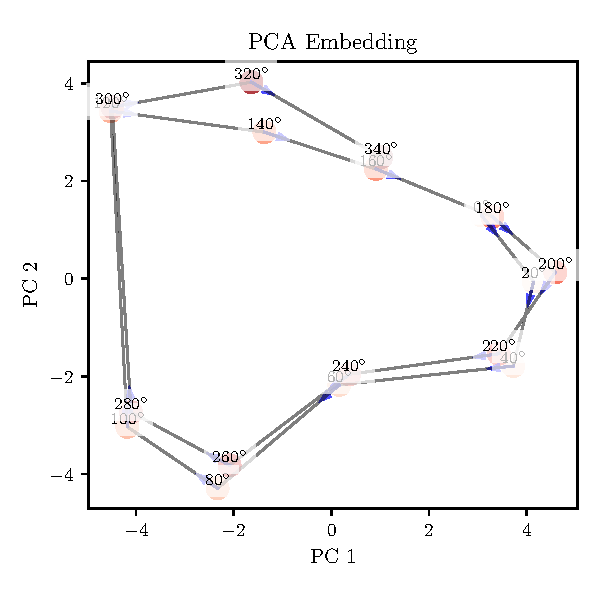
\includegraphics[width=\textwidth]{results/mouse_circular_colormap_visualization.pdf}
        % \caption{Circular colormap visualization of the latent space, showing how orientation angles map continuously onto the manifold.}
        \label{fig:mouse_colormap}
    \end{subfigure}
    \hfill
    \begin{subfigure}[b]{0.48\textwidth}
        \centering
        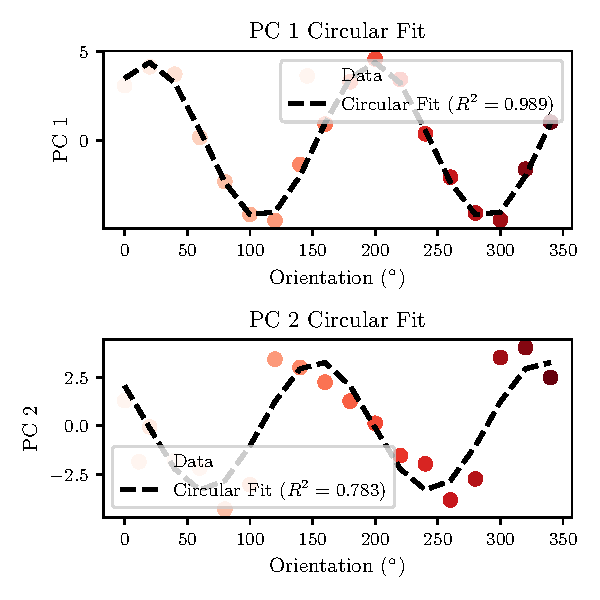
\includegraphics[width=\textwidth]{results/mouse_circular_regression.pdf}
        % \caption{Circular regression analysis demonstrating the relationship between true orientation angles and their position on the manifold.}
        \label{fig:mouse_regression}
    \end{subfigure}

    \label{fig:mouse_manifold_analysis}
\end{figure}

\section{Simulation Study}

To demonstrate the emergence of geometric structures in neural representations of ANNs, we implemented a simulation experiment investigating how ANNs encode ``circular variables''. This experiment provides an example of neural population geometry principles and illustrates how topological structures may naturally emerge in neural representations in response to the nature of the task.


We trained a CNN to predict the angle of orientation, $\theta$, of visual grating stimuli, a task analogous to orientation selectivity in the visual cortex. The network was presented with sinusoidal gratings at various orientations ranging from 0 to $2\pi$ rad and tasked with predicting the orientation angle. Fig. \ref{fig:grating_samples} contains example stimuli.

\begin{figure}
    \centering
    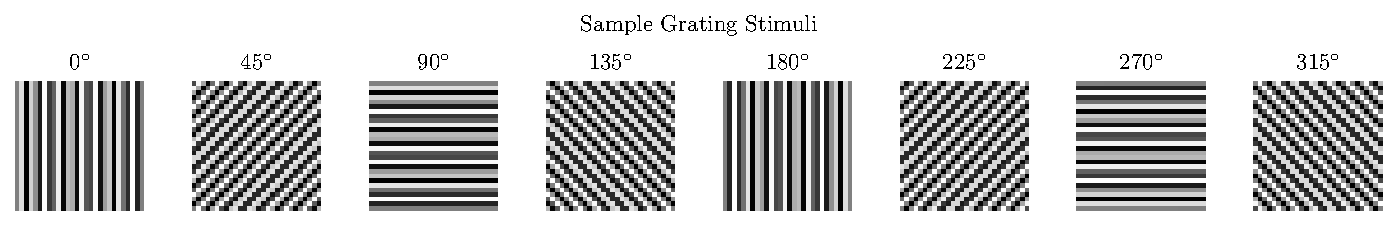
\includegraphics[width=\linewidth]{results/grating_samples.pdf}
    \caption{Sample grating stimuli at different orientations.}
    \label{fig:grating_samples}
\end{figure}

The architecture consisted of convolutional layers followed by fully connected layers, with a 388-dimensional latent space that we analyzed for geometric properties. Importantly, the network was trained to predict the sine and cosine components of the orientation angle rather than the raw angle, which naturally handles the circular topology of the orientation space\footnote{For example, for small $\epsilon$, the angles of $\epsilon$ and $2\pi - \epsilon$ are nearly identical orientations but numerically distant. Using sine-cosine encoding, these angles map to points $(\cos(\epsilon), \sin(\epsilon)) \approx (\cos(2\pi-\epsilon), \sin(2\pi - \epsilon)) \approx (1, 0)$, i.e., the orientations become close in Euclidean space, better reflecting their similarity.}.

\begin{figure}
    \centering
    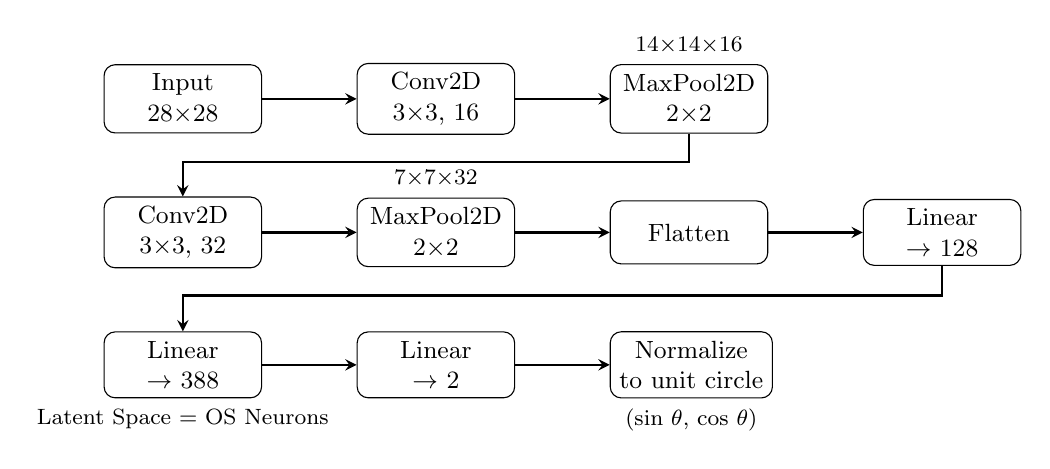
\begin{tikzpicture}[
        node distance=1.2cm,
        box/.style={
            rectangle,
            draw,
            minimum width=2cm,
            minimum height=0.8cm,
            align=center,
            rounded corners,
            font=\small
        },
        arrow/.style={
            ->,
            thick,
            >=stealth
        }
    ]

    % Input layer
    \node[box] (input) {Input\\28$\times$28};

    % First conv block
    \node[box, right=of input] (conv1) {Conv2D\\3$\times$3, 16};
    \node[box, right=of conv1] (pool1) {MaxPool2D\\2$\times$2};

    % Second conv block
    \node[box, below=0.8cm of input] (conv2) {Conv2D\\3$\times$3, 32};
    \node[box, right=of conv2] (pool2) {MaxPool2D\\2$\times$2};

    % Flatten and FC layers
    \node[box, right=of pool2] (flatten) {Flatten};
    \node[box, right=of flatten] (fc1) {Linear\\$\rightarrow$ 128};
    
    % Second row of FC layers
    \node[box, below=0.8cm of conv2] (fc2) {Linear\\$\rightarrow$ 388};
    \node[box, right=of fc2] (output_raw) {Linear\\$\rightarrow$ 2};
    \node[box, right=of output_raw] (output_norm) {Normalize\\to unit circle};

    % Connections - modified to create column-like flow
    \draw[arrow] (input) -- (conv1);
    \draw[arrow] (conv1) -- (pool1);
    
    % Modified connections to go down and then across instead of diagonal
    \draw[arrow] (pool1) -- ++(0,-0.8cm) -| (conv2);
    \draw[arrow] (conv2) -- (pool2);
    \draw[arrow] (pool2) -- (flatten);
    \draw[arrow] (flatten) -- (fc1);
    
    % Modified connection to go down and then across
    \draw[arrow] (fc1) -- ++(0,-0.8cm) -| (fc2);
    \draw[arrow] (fc2) -- (output_raw);
    \draw[arrow] (output_raw) -- (output_norm);

    % Add dimensions as labels
    \node[above=0.01cm of pool1, font=\footnotesize] {14$\times$14$\times$16};
    \node[above=0.01cm of pool2, font=\footnotesize] {7$\times$7$\times$32};
    \node[below=0.01cm of fc2, font=\footnotesize] {Latent Space  = OS Neurons};
    \node[below=0.01cm of output_norm, font=\footnotesize] {(sin $\theta$, cos $\theta$)};

    \end{tikzpicture}
    \caption{Neural network architecture used for the circular manifold experiment. The network processes grating stimuli through convolutional layers, followed by fully connected layers that produce a 388-dimensional latent space. The output layer predicts raw values that are then normalized to the unit circle to represent the sine and cosine of the orientation angle, ensuring the circular topology is preserved.}
\end{figure}

After training, we extracted the 388-dimensional latent representations for test stimuli and PCA to visualize the structure of these representations. The results revealed a striking circular manifold in the latent space, where stimuli with similar orientations were positioned close together, and the entire orientation space was represented as a continuous ring.

\begin{figure}
    \centering
    \begin{subfigure}[b]{0.48\textwidth}
        \centering
        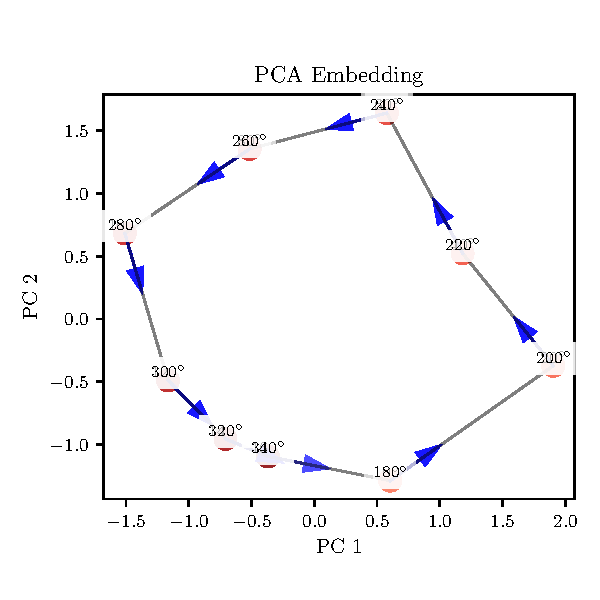
\includegraphics[width=\textwidth]{results/ann_circular_colormap_visualization.pdf}
        % \caption{Circular colormap visualization of the latent space, showing how orientation angles map continuously onto the manifold.}
        \label{fig:circular_colormap}
    \end{subfigure}
    \hfill
    \begin{subfigure}[b]{0.48\textwidth}
        \centering
        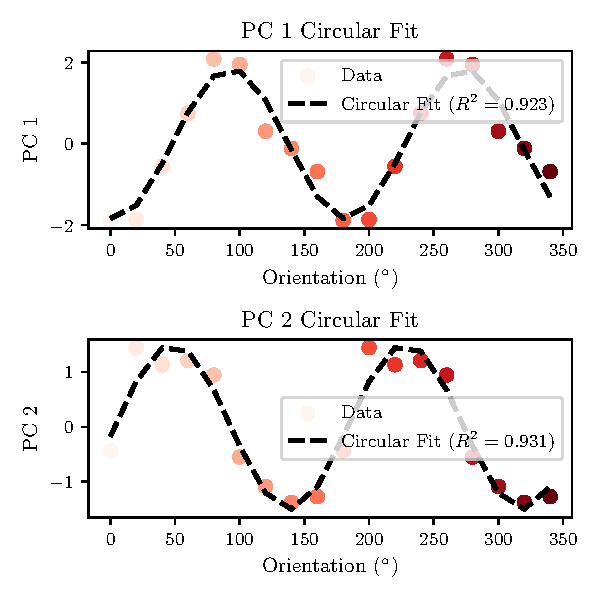
\includegraphics[width=\textwidth]{results/ann_circular_regression.pdf}
        % \caption{Circular regression analysis demonstrating the relationship between true orientation angles and their position on the manifold.}
        \label{fig:circular_regression}
    \end{subfigure}
    \caption{Analysis of the circular manifold in the CNN's latent space. The network spontaneously learns to represent orientation as a ring-shaped manifold, where similar orientations are positioned close together and the full range of orientations forms a closed loop. This geometric structure emerges naturally from the training process, reflecting the circular topology of the orientation space. The continuous mapping between orientation angles and positions on the manifold demonstrates how the network has learned to encode this periodic variable in a topologically appropriate manner.}
    \label{fig:manifold_analysis}
\end{figure}

This circular topology emerged naturally from the training process, despite no explicit topological constraints being imposed on the network. Through backpropagation, the network discovered that a circular representation is the most efficient way to encode a periodic variable, demonstrating how the geometry of the task space (in this case, the circular nature of orientation angles) becomes reflected in the geometry of the neural representations.

The experiment highlights several key principles of neural population geometry. First, the network's internal representations form a low-dimensional manifold (a circle) embedded in the high-dimensional latent space. Second, the topology of the manifold (circular) matches the topology of the task space (orientation angles), demonstrating topological correspondence. Third, similar stimuli are mapped to nearby points on the manifold, preserving the continuity of the input space through continuous representation. Finally, the network learns to compress the high-dimensional input (grating images) into a low-dimensional representation that captures the essential variable (orientation), effectively performing dimensionality reduction.

This simple experiment provides an intuitive foundation for understanding how more complex neural networks might represent more complicated manifolds in their latent spaces, and how the geometry of these representations relates to the computational tasks being performed.

\section{Conclusion}

\bibliographystyle{unsrt}
\bibliography{refs}

\end{document}
